\subsection{Thời gian: Sắp xếp theo trình tự thời gian tuyến tính}
Một trong những cách đơn giản nhất để biểu diễn dữ liệu chuỗi thời gian là sử dụng hệ tọa độ Descartes với trục hoành thể hiện mốc thời gian và trục tung thể hiện giá trị biến định lượng tương ứng. Mỗi cặp gồm mốc thời gian và giá trị tương ứng được thể hiện bằng một điểm trên hệ tọa độ. Cách biểu diễn này thường được gọi là \textit{đồ thị điểm}, \textit{biểu đồ điểm}, hoặc \textit{biểu đồ phân tán} (scatterplot). Harris [170] mô tả cách biểu diễn này là một dạng đồ thị hai chiều trong đó độ lớn của các biến định lượng được thể hiện thông qua khoảng cách của mỗi điểm đến các trục tọa độ. Ngoài dạng cơ bản này còn có nhiều biến thể mở rộng khác, chẳng hạn như kỹ thuật 3D (biểu đồ lớp) hoặc kỹ thuật sử dụng nhiều ký hiệu khác nhau thay vì chỉ đơn thuần là các điểm giống nhau. Kỹ thuật này đặc biệt phù hợp trong trường hợp muốn nhấn mạnh từng giá trị riêng lẻ. Bên cạnh đó, việc biểu diễn dữ liệu bằng các thang đo chung thống nhất sẽ giúp cho người đọc có thể dễ dàng nắm bắt được thông tin một cách trực quan và chính xác nhất. 
\\ \\
Phát triển trên nền tảng của biểu đồ điểm, \textit{biểu đồ đường} cho phép ta thể hiện được mối liên hệ về mặt thời gian giữa các điểm dữ liệu thông qua việc gắn các điểm dữ liệu đó trên một đường nối. Khác với biểu đồ điểm khi tập trung nhấn mạnh vào các điểm dữ liệu riêng lẻ, rời rạc, biều đồ đường sẽ giúp ta tập trung vào xu hướng tổng quan của dữ liệu theo thời gian. Tùy thuộc vào đối tượng đang được xem xét đến ta có thể sử dụng các kiểu kết nối khác nhau giữa các điểm dữ liệu như: đường thẳng, đường bậc thang (liên tục thay đổi giá trị) hoặc đường cong Bezier. Tuy nhiên, dù sử dụng bất kỳ kiểu kết nối nào nêu trên cũng cần lưu ý rằng việc phản ánh giá trị của các điểm nằm giữa hai điểm dữ liệu đã biết đều chỉ mang tính tương đối và ta sẽ không thể đảm bảo chắc chắn về độ chính xác cho mọi điểm dữ liệu được thể hiện trên đường nối. Một vấn đề khác cần lưu ý là việc thiếu dữ liệu. Trong các trường hợp thiếu dữ liệu của một khoảng thời gian nhất định mà người phân tích bỏ qua yếu tố này và chỉ đơn thuần kết nối các điểm dữ liệu liền trước và liền sau khoảng thời gian đó thì nhiều khả năng sẽ dẫn đến những kết luận không chính xác. Do đó, cần có cách thức phù hợp để biểu diễn cho người xem ý thức được vấn đề này, chẳng hạn bằng cách sử dụng các đường nối bằng nét đứt. 
\\ \\ 
Bên cạnh các dạng biểu đồ nêu trên, ta có thể sử dụng một số dạng mở rộng và biến thể khác như: biểu đồ nhiệt, biểu đồ dải, biểu đồ đường lớp, biểu đồ miền, biểu đồ chỉ số hoặc biểu đồ kiểm soát (còn gọi là biểu đồ hành vi – quy trình) (xem [170]).   
\begin{figure}[H] % places figure environment here   
    \centering % Centers Graphic
    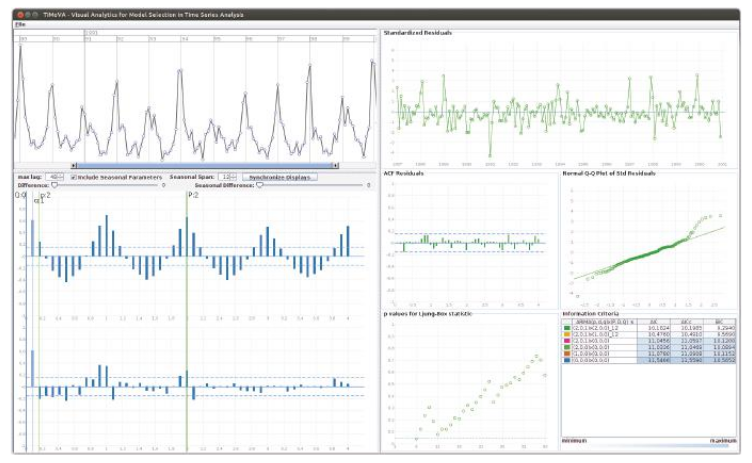
\includegraphics[width=0.8\textwidth]{assets/fig_7_8.png} 
    \caption{iMoVA. Giao diện thể hiện biểu đồ chuỗi thời gian dưới dạng biểu đồ đường (dữ liệu đầu vào; trên cùng bên trái), công cụ lựa chọn mô hình và nhiều chế độ xem khác để định hướng, hỗ trợ quá trình lựa chọn mô hình. (Nguồn: Thực hiện bằng phần mềm nguyên mẫu TiMoVA.)} % Creates caption underneath graph
    \label{fig:f7.8}
\end{figure}
Các loại biểu đồ điểm, biểu đồ đường cũng như các biểu đồ trực quan hóa khác (ví dụ: biểu đồ cột) được sử dụng một cách thường xuyên trong quá trình \textit{TiMoVA (“Ti”: Time series analysis - Phân tích chuỗi thời gian, “Mo”: Model selection - Lựa chọn mô hình, “VA”: applies Visual Analytics methods - áp dụng các phương pháp Phân tích hình ảnh trực quan)} [42]. Phân tích thống kê với dữ liệu chuỗi thời gian là một nhiệm vụ đầy thách thức và đòi hỏi phải được thực hiện bởi các chuyên gia trong nhiều lĩnh vực khác nhau, ví dụ như khi một nhân viên y tế công muốn dự đoán số người cần được điều trị tim mạch trong năm tới. Thông thường, việc lựa chọn mô hình là một nhiệm vụ phức tạp. Chính vì vậy, TiMoVA là một công cụ hữu hiệu, cung cấp giao diện tương tác để định hướng cho người dùng khai phá dữ liệu và lựa chọn mô hình chuỗi thời gian phù hợp. TiMoVA hỗ trợ chuyên gia trong các lĩnh vực ngành nghề trong việc: (1) lựa chọn thứ tự mô hình tương tác thông qua một giao diện trực quan, (2) cung cấp phản hồi về kết quả mô hình trong quá trình chọn thứ tự mô hình một cách trực quan và nhanh chóng tức thì, (3) quyết định về việc có nên cải thiện, thay đổi mô hình hay không (Hình 7.8). Một đánh giá thực nghiệm sử dụng bộ dữ liệu dịch tễ và sự tham gia đánh giá của 02 (hai) chuyên gia thống kê cho thấy TiMoVA hỗ trợ rất hiệu quả trong việc tạo ra một môi trường tương tác khám phá dữ liệu từ đó giúp lựa chọn được các mô hình phù hợp.